\documentclass[tikz]{standalone}
\usepackage{pgfplots}
\pgfplotsset{compat=1.15}
\usepackage{mathrsfs}
\usetikzlibrary{arrows,calc}
\usepackage{tkz-euclide}
\pagestyle{empty}

\definecolor{AngleClr}{rgb}{0,0.39215686274509803,0}
\definecolor{ShapeClr}{rgb}{0.6,0.2,0}
\definecolor{BlueClr}{RGB}{5,81,163}

\begin{document}

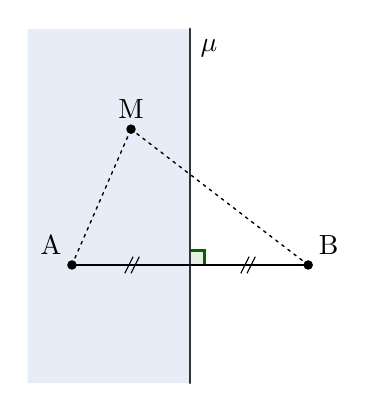
\begin{tikzpicture}[scale=.75]
\tkzSetUpLine[line width=1pt,color=black]
\tkzSetUpPoint[fill=black]

\tkzDefPoints{0/0/A,4/0/B,2/4/C,2/-2/D,2/0/O}
\tkzDefPoints{-0.75/4/AC,-0.75/-2/AD,1/2.3/M}

\tkzMarkRightAngle[line width=1pt, size=.25,color=AngleClr,fill=AngleClr,fill opacity=0.1](C,O,B)

\tkzFillPolygon[fill=BlueClr,fill opacity=0.1](C,D,AD,AC)

\tkzDrawSegment[line width=0.8pt,color=black!80!white](C,D)
\tkzDrawSegment[line width=1.0pt,color=black](A,B)

\tkzDrawSegments[line width=0.5pt,color=black,dashed,dash pattern=on 1pt off 1.75pt](A,M B,M)
\tkzDrawPoints[size=3](A,B,M)

\tkzLabelPoint[above left](A){$\rm A$}
\tkzLabelPoint[above right](B){$\rm B$}
\tkzLabelPoint[above](M){$\rm M$}

\tkzLabelSegments[pos=0.0,below right](C,D){$\mu$}

\tkzMarkSegments[mark=s||,size=3](A,O B,O)

\end{tikzpicture}
\end{document}
